\documentclass[a4paper, 12pt, twoside]{article}


%------------------------------------------------------------------------
%
% Author                :   Lasercata
% Last modification     :   2022.05.25
%
%------------------------------------------------------------------------


%------ini
\usepackage[utf8]{inputenc}
\usepackage[T1]{fontenc}
\usepackage[french]{babel}
%\usepackage[english]{babel}


%------geometry
\usepackage[textheight=700pt, textwidth=500pt]{geometry}


%------color
\usepackage{xcolor}
\definecolor{ff4500}{HTML}{ff4500}
\definecolor{00f}{HTML}{0000ff}
\definecolor{0ff}{HTML}{00ffff}
\definecolor{656565}{HTML}{656565}

\renewcommand{\emph}{\textcolor{ff4500}}
\renewcommand{\em}{\color{ff4500}}

\newcommand{\strong}[1]{\textcolor{ff4500}{\bf #1}}
\newcommand{\st}{\color{ff4500}\bf}


%------Code highlighting
%---listings
\usepackage{listings}

\definecolor{cbg}{HTML}{272822}
\definecolor{cfg}{HTML}{ececec}
\definecolor{ccomment}{HTML}{686c58}
\definecolor{ckw}{HTML}{f92672}
\definecolor{cstring}{HTML}{e6db72}
\definecolor{cstringlight}{HTML}{98980f}
\definecolor{lightwhite}{HTML}{fafafa}

\lstdefinestyle{DarkCodeStyle}{
    backgroundcolor=\color{cbg},
    commentstyle=\itshape\color{ccomment},
    keywordstyle=\color{ckw},
    numberstyle=\tiny\color{cbg},
    stringstyle=\color{cstring},
    basicstyle=\ttfamily\footnotesize\color{cfg},
    breakatwhitespace=false,
    breaklines=true,
    captionpos=b,
    keepspaces=true,
    numbers=left,
    numbersep=5pt,
    showspaces=false,
    showstringspaces=false,
    showtabs=false,
    tabsize=4,
    xleftmargin=\leftskip
}

\lstdefinestyle{LightCodeStyle}{
    backgroundcolor=\color{lightwhite},
    commentstyle=\itshape\color{ccomment},
    keywordstyle=\color{ckw},
    numberstyle=\tiny\color{cbg},
    stringstyle=\color{cstringlight},
    basicstyle=\ttfamily\footnotesize\color{cbg},
    breakatwhitespace=false,
    breaklines=true,
    captionpos=b,
    keepspaces=true,
    numbers=left,
    numbersep=10pt,
    showspaces=false,
    showstringspaces=false,
    showtabs=false,
    tabsize=4,
    frame=L,
    xleftmargin=\leftskip
}

%\lstset{style=DarkCodeStyle}
\lstset{style=LightCodeStyle}
%Usage : \begin{lstlisting}[language=Caml] ... \end{lstlisting}

%---tcolorbox
\usepackage[many]{tcolorbox}
\DeclareTColorBox{pseudocode}{O{black}O{lightwhite}}{
    breakable,
    outer arc=0pt,
    arc=0pt,
    top=0pt,
    toprule=-.5pt,
    right=0pt,
    rightrule=-.5pt,
    bottom=0pt,
    bottomrule=-.5pt,
    colframe=#1,
    colback=#2,
    enlarge left by=10pt,
    width=\linewidth-\leftskip-10pt,
}


%-------make the table of content clickable
\usepackage{hyperref}
\hypersetup{
    colorlinks,
    citecolor=black,
    filecolor=black,
    linkcolor=black,
    urlcolor=black
}
%Uncomment this and comment above for dark mode
% \hypersetup{
%     colorlinks,
%     citecolor=white,
%     filecolor=white,
%     linkcolor=white,
%     urlcolor=white
% }


%------pictures
\usepackage{graphicx}
%\usepackage{wrapfig}

\usepackage{tikz}
%\usetikzlibrary{babel}             %Uncomment this to use circuitikz
%\usetikzlibrary{shapes.geometric}  % To draw triangles in trees
%\usepackage{circuitikz}            %Electrical circuits drawing


%------tabular
%\usepackage{color}
%\usepackage{colortbl}
%\usepackage{multirow}


%------Physics
%---Packages
%\usepackage[version=4]{mhchem} %$\ce{NO4^2-}$

%---Commands
\newcommand{\link}[2]{\mathrm{#1} \! - \! \mathrm{#2}}
\newcommand{\pt}[1]{\cdot 10^{#1}} % Power of ten
\newcommand{\dt}[2][t]{\dfrac{\mathrm d #2}{\mathrm d #1}} % Derivative


%------math
%---Packages
%\usepackage{textcomp}
%\usepackage{amsmath}
\usepackage{amssymb}
\usepackage{mathtools} % For abs
\usepackage{stmaryrd} %for \llbracket and \rrbracket
\usepackage{mathrsfs} %for \mathscr{x} (different from \mathcal{x})

%---Commands
%-Sets
\newcommand{\N}{\mathbb{N}} %set N
\newcommand{\Z}{\mathbb{Z}} %set Z
\newcommand{\Q}{\mathbb{Q}} %set Q
\newcommand{\R}{\mathbb{R}} %set R
\newcommand{\C}{\mathbb{C}} %set C
\newcommand{\U}{\mathbb{U}} %set U
\newcommand{\seg}[2]{\left[ #1\ ;\ #2 \right]}
\newcommand{\nset}[2]{\left\llbracket #1\ ;\ #2 \right\rrbracket}

%-Exponantial / complexs
\newcommand{\e}{\mathrm{e}}
\newcommand{\cj}[1]{\overline{#1}} %overline for the conjugate.

%-Vectors
\newcommand{\vect}{\overrightarrow}
\newcommand{\veco}[3]{\displaystyle \vect{#1}\binom{#2}{#3}} %vector + coord

%-Limits
\newcommand{\lm}[2][{}]{\lim\limits_{\substack{#2 \\ #1}}} %$\lm{x \to a} f$ or $\lm[x < a]{x \to a} f$
\newcommand{\Lm}[3][{}]{\lm[#1]{#2} \left( #3 \right)} %$\Lm{x \to a}{f}$ or $\Lm[x < a]{x \to a}{f}$
\newcommand{\tendsto}[1]{\xrightarrow[#1]{}}

%-Integral
\newcommand{\dint}[4][x]{\displaystyle \int_{#2}^{#3} #4 \mathrm{d} #1} %$\dint{a}{b}{f(x)}$ or $\dint[t]{a}{b}{f(t)}$

%-left right
\newcommand{\lr}[1]{\left( #1 \right)}
\newcommand{\lrb}[1]{\left[ #1 \right]}
\newcommand{\lrbb}[1]{\left\llbracket #1 \right\rrbracket}
\newcommand{\set}[1]{\left\{ #1 \right\}}
\newcommand{\abs}[1]{\left\lvert #1 \right\rvert}
\newcommand{\ceil}[1]{\left\lceil #1 \right\rceil}
\newcommand{\floor}[1]{\left\lfloor #1 \right\rfloor}
\newcommand{\lrangle}[1]{\left\langle #1 \right\rangle}

%-Others
\newcommand{\para}{\ /\!/\ } %//
\newcommand{\ssi}{\ \Leftrightarrow \ }
\newcommand{\eqsys}[2]{\begin{cases} #1 \\ #2 \end{cases}}

\newcommand{\med}[2]{\mathrm{med} \left[ #1\ ;\ #2 \right]}  %$\med{A}{B} -> med[A ; B]$
\newcommand{\Circ}[2]{\mathscr{C}_{#1, #2}}

\renewcommand{\le}{\leqslant}
\renewcommand{\ge}{\geqslant}

\newcommand{\oboxed}[1]{\textcolor{ff4500}{\boxed{\textcolor{black}{#1}}}} %orange boxed


%------commands
%---to quote french text
\newcommand{\simplecit}[1]{\guillemotleft$\;$#1$\;$\guillemotright}
\newcommand{\cit}[1]{\simplecit{\textcolor{656565}{#1}}}
\newcommand{\quo}[1]{\cit{\it #1}}

%---to indent
\newcommand{\ind}[1][20pt]{\advance\leftskip + #1}
\newcommand{\deind}[1][20pt]{\advance\leftskip - #1}

%---to indent a text
\newcommand{\indented}[2][20pt]{\par \ind[#1] #2 \par \deind[#1]}
\newenvironment{indt}[2][20pt]{#2 \par \ind[#1]}{\par \deind} %Titled indented env

%---title
\newcommand{\thetitle}[2]{\begin{center}\textbf{{\LARGE \underline{\emph{#1} :}} {\Large #2}}\end{center}}


%------Sections
% To change section numbering :
% \renewcommand\thesection{\Roman{section}}
% \renewcommand\thesubsection{\arabic{subsection}}
% \renewcommand\thesubsubsection{\textit \alph{subsubsection}}

% To start numbering from 0
% \setcounter{section}{-1}


%------page style
\usepackage{fancyhdr}
\usepackage{lastpage}

\setlength{\headheight}{18pt}
\setlength{\footskip}{50pt}

\pagestyle{fancy}
\fancyhf{}
\fancyhead[LE, RO]{\textit{\textcolor{black}{\today}}}
\fancyhead[RE, LO]{\large{\textsl{\emph{\texttt{\jobname}}}}}

\fancyfoot[RO, LE]{\textit{\texttt{\textcolor{black}{Page \thepage /}\pageref{LastPage}}}} %Change 'black' to 'white' for dark mode
\fancyfoot[LO, RE]{\includegraphics[scale=0.12]{/home/lasercata/Pictures/1.images_profil/logo/mieux/lasercata_logo_fly_fond_blanc.png}}

% For dark mode :
%/home/lasercata/Pictures/1.images_profil/logo/mieux/lasercata_logo_fly.png


%------init lengths
\setlength{\parindent}{0pt} %To avoid using \noindent everywhere.
\setlength{\parskip}{3pt}


%---------------------------------Begin Document
\begin{document}
    
    %For dark mode :
    % \pagecolor{black}
    % \color{white}
    
    \thetitle{Chapitre 10}{Théorie des graphes}
    
    \tableofcontents
    \newpage
    
    
    \begin{indt}{\section{Introduction}}
        
        \begin{indt}{\subsection{Les origines}}
            \begin{indt}{\subsubsection{Le problème fondateur : les sept ponts de Königsberg}}
                \label{1.1.1}

                \textit{\'Enoncé} : Peut-on effectuer une promenade à Königsberg passant exactement une fois par chacun des ponts ?

                Variante : peut-on le faire en revenant à son point de départ ?

                \begin{center}
                    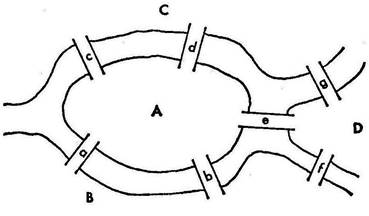
\includegraphics[scale=.5]{pics/pic_1.jpg}
                \end{center}
            \end{indt}

            \vspace{12pt}
            
            \begin{indt}{\subsubsection{Une solution formelle}}
                Présentée par \textsc{Euler} en 1735.

                \begin{indt}{Trois étapes :}
                    (1) Nommage des trois zones et représentation abstraite

                    \begin{center}
                        \begin{tikzpicture}[node distance = 50pt]
                            \node (A) [circle, draw] {A};
                            \node (B) [circle, draw, below right of = A] {B};
                            \node (C) [circle, draw, above right of = A] {C};
                            \node (D) [circle, draw, below right of = C] {D};

                            \draw (A) -- (C) -- (D) -- (B) -- (A);
                            \draw (A) -- (D);

                            \draw (A) to [out=90, in=180] (C);
                            \draw (A) to [out=-90, in=-180] (B);
                        \end{tikzpicture}
                    \end{center}

                    (2) Formalisation de la notion de chemin

                    (3) Démonstration d'impossibilité : il n'existe pas de chemin / circuit eulérien dans ce graphe.
                \end{indt}
            \end{indt}

            \vspace{12pt}
            
            \begin{indt}{\subsubsection{Remarque}}
                Les points (1) et (2) sont les étapes fondatrices de la théorie des graphes vue comme une théorie mathématique.
                Cette théorie a pris une grande ampleur car elle permet de modéliser de nombreux phénomènes.
            \end{indt}
        \end{indt}

        \vspace{12pt}
        
        \begin{indt}{\subsection{De nombreuses applications}}
            \begin{indt}{\subsubsection{Compilation}}
                $\bullet$ Modélisation : on représente le graphe de dépendance entre fichiers.

                \begin{center}
                    \begin{tikzpicture}
                        \node (f) at (0, 0) [rectangle, draw] {
                            \begin{tabular}{l}
                                Foo.ml
                                \\
                                \fbox{open Bar}
                            \end{tabular}
                        };

                        
                        \node (b) at (4, 0) [rectangle, draw] {
                            \begin{tabular}{l}
                                Bar.ml
                                \\
                                \fbox{open Foo}
                            \end{tabular}
                        };

                        \draw[->] (b) to [in=10, out=170] (f);
                        \draw[<-] (b) to [in=-10, out=-170] (f);
                    \end{tikzpicture}
                \end{center}

                $\bullet$ Problème : faisabilité : c'est un problème de détection de cycle.

                Ordre de compilation : choisir un ordre, c'est effectuer un tri topologique du graphe.
            \end{indt}

            \vspace{12pt}
            
            \begin{indt}{\subsubsection{Transports}}
                \label{1.2.2}
                
                $\bullet$ Modélisation : on représente un réseau de transports en commun en représentant les stations liées par les lignes qui y passent.

                $\bullet$ Problème : recherche de chemin le plus court en terme de distance / de temps / nombre de stations.
            \end{indt}

            \vspace{12pt}
            
            \begin{indt}{\subsubsection{Ordonnancement de tâches}}
                $\bullet$ Problème : répartition d'un ensemble de tâches sur un nombre minimal d'unité de calcul.

                $\bullet$ Modélisation : on utilise un graphe d'incompatibilité : on lie les tâches incompatibles entre elles. On veut attribuer une couleur (une unité de calcul) à chaque sommet de sorte qu'aucun sommet ne soit de la même couleur que l'un de ses voisins.
            \end{indt}

            \vspace{12pt}
            
            \begin{indt}{\subsubsection{Construction d'un réseau électrique}}
                \label{1.2.4}
                
                $\bullet$ Problème : on veut raccorder un certain nombre de villes en utilisant le moins de câble possible.

                $\bullet$ Modélisation : on utilise un graphe qui représente les villes liées par des axes annotés par leur longueur. On veut sélectionner des axes pour lier toutes les villes entre elles en utilisant le moins de longueur possible.

                C'est la recherche d'un arbre couvrant de poids minimal.
            \end{indt}
        \end{indt}
        
    \end{indt}

    \vspace{12pt}
    
    \begin{indt}{\section{Bases des graphes}}
        \begin{indt}{\subsection{Vocabulaire}}
            \begin{indt}{\subsubsection{Définition (\textit{graphe})}}
                \begin{indt}{Un graphe est un couple $G = (S, A)$ où :}
                    \label{2.1.1}

                    $\bullet$ $S$ est un ensemble fini de \textit{sommets} ou de \textit{n\oe uds} ;

                    \begin{indt}{$\bullet$ $A$ est un ensemble d'associations entre deux sommets, qui peut prendre plusieurs formes :}
                        $-$ Si $A$ est un ensemble de points de sommets, on dit que $G$ est \textit{non orienté} ;

                        $-$ Si $a = \set{s, s'} \in A$ , on dit que $a$ est une \textit{arête} d'extrémités $s$ et $s'$, que $a$ est \textit{incidente} à $s$ et $s'$, et que $s$ et $s'$ sont \textit{adjacents} ou \textit{voisins} ;

                        $-$ Si $A$ est un ensemble de couples de sommets, on dit que $G$ est \textit{orienté}.
                        \newline
                        Si $a = (s, s') \in A$, on dit que $a$ est un \textit{arc}, que $s'$ est un \textit{successeur} de $s$, que $a$ est un \textit{arc sortant} pour $s$ et \textit{entrant} pour $s'$.
                    \end{indt}
                \end{indt}
            \end{indt}

            \vspace{12pt}
            
            \begin{indt}{\subsubsection{Représentation graphique}}
                On place un point pour chaque sommet et on relie les extrémités d'une même arête (avec une flèche dans le cas orienté).

                Exemple :
                \[
                    G = \lr{\set{A, B, C, D}, \set{\set{A, B}, \set{B, C}, \set{C, A}}}
                \]

                est un graphe non orienté (GNO)

                \begin{center}
                    \begin{tikzpicture}[node distance = 40pt]
                        \node (A) [circle, draw] {A};
                        \node (B) [circle, draw, above right of = A] {B};
                        \node (C) [circle, draw, below right of = A] {C};
                        \node (D) [circle, draw, below right of = B] {D};

                        \draw (A) -- (B) -- (C) -- (A);
                    \end{tikzpicture}
                \end{center}

                Autre exemple :

                \begin{center}
                    \begin{tikzpicture}[node distance = 40pt]
                        \node (A) [circle, draw] {A};
                        \node (B) [circle, draw, right of = A] {B};
                        \node (C) [circle, draw, above of = B] {C};
                        \node (D) [circle, draw, right of = B] {D};

                        \draw[->] (A) to [out=10, in=170] (B);
                        \draw[<-] (A) to [out=-10, in=-170] (B);
                        \draw[->] (D) -- (B);
                        \draw[->] (B) -- (C);
                        \draw[->] (A) to [out=-40, in=-140] (D);
                        \draw[->] (A) -- (C);
                        \draw[->] (C) -- (D);
                    \end{tikzpicture}
                \end{center}

                est la représentation du graphe orienté (GO) :
                \[
                    G = \lr{ \set{A,B,C,D}, \set{(A, B), (B, A), (B, C), (D, B), (A, D), (A, C), (C, D)} }
                \]
                
            \end{indt}

            \vspace{12pt}
            
            \begin{indt}{\subsubsection{Boucles}}
                $\bullet$ Définition (\textit{boucle}) : Une \textit{boucle} dans un graphe est une arête / un arc dont les extrémités sont égales.

                $\bullet$ Remarque : la définition \ref{2.1.1} (page \pageref{2.1.1}) empêche la présence de boucles dans les GNO.
                On peut les autoriser en considérant non pas des paires de sommets, mais des \textit{multi-ensembles} de cardinal 2.

                On pourrait aussi utiliser les \textit{multi-ensembles} pour autoriser les multi-arêtes (plusieurs arêtes entre 2 sommets donnés, comme ent \ref{1.1.1}, page \pageref{1.1.1}, mais c'est H.P : $A$ sera toujours un ensemble).
            \end{indt}

            \vspace{12pt}
            
            \begin{indt}{\subsubsection{Degré}}
                $\bullet$ Définition (\textit{degré}) : Soit $G = (S, A)$ un GNO et $s \in S$.

                Le degré de $s$, noté $d(s)$  est le nombre de voisins de $s$ :
                \[
                    d(s) = \abs{\vphantom{\dfrac a a}\!\set{a \in A\ |\ s \in a}}
                \]
                
                $\bullet$ Définition (\textit{degré entrant / sortant}) : Soit $G = (S, A)$ un GO et $s \in S$.

                Le \textit{degré entrant} (resp. \textit{sortant}) de $s$, noté $d_-(s)$  (resp. $d_+(s)$), est le nombre d'arcs entrants (resp. sortant) pour $s$ :
                \[
                    d_-(s) = \abs{\vphantom{\dfrac a a}\!\set{a \in A\ |\ \exists s' \in S\ |\ a = (s', s)}}
                \]
                \[
                    d_+(s) = \abs{\vphantom{\dfrac a a}\!\set{a \in A\ |\ \exists s' \in S\ |\ a = (s, s')}}
                \]
                
                \begin{indt}{$\bullet$ Proposition (formule de la somme des degrés) : Soit $G = (S, A)$ un graphe.}
                    (1) Si $G$ est un GNO sans boucle,
                    \[
                        \sum_{s \in S} d(s) = 2\abs{A}
                    \]

                    (2) Si $G$ est un GO,
                    \[
                        \sum_{s \in S} d_-(s) = \sum_{s \in S} d_+(s) = \abs{A}
                    \]
                \end{indt}

                \begin{indt}{$\square$ Démonstration :}
                    (1) On compte les extrémités d'arêtes :

                    $-$ Une arête compte pour deux extrémités car ce n'est pas une boucle, donc il y en a $2\abs A$ ;

                    $-$ $\forall s \in S$, $s$ est extrémité de $d(s)$ arêtes, donc il y en a
                    \[
                        \sum_{s \in S} d(s)
                    \]
                    
                    (2) Par récurrence sur $\abs A$ :

                    $-$ Si $\abs A = 0,\ \forall s \in S,\ d_+(s) = d_-(s) = 0$ : ok.

                    $-$ Héréditée : si $\abs A > 0$, alors $\exists (s, s') \in A$.

                    On note $G' = (S,\ A \setminus \set{(s, s')})$.

                    Par hypothèse de récurrence :
                    \[
                        \abs A - 1 = \abs{A \setminus \set{(s, s')}} = \sum_{v \in S \setminus \set{s'}} d_-(v) + \underbrace{d_-(s) - 1}_{\text{degré sortant de $s$ dans $G$}}
                    \]
                    
                    Donc $\abs A = \displaystyle \sum_{v \in S} d_-(v)$

                    De même pour les degrés entrants, en considérant $s'$ plutôt que $s$
                    $\blacksquare$
                \end{indt}

                \vspace{6pt}
                
                $\bullet$ Corollaire (\textit{handshaking lemma}) : Tout GNO sans boucle possède un nombre pair de sommets de degré impair.

                \begin{indt}{$\square$ Démonstration :}
                    \[
                        2\N \ni 2\abs A
                        = \sum_{s \in S} d(s)
                        = \underbrace{\sum_{\substack{s \in S \\ d(s) \in 2\N}} d(s)}_{\in 2\N} + \underbrace{\sum_{\substack{s \in S \\ d(s) \in 2\N + 1}} d(s)}_{\substack{\text{de la parité du nombre} \\ \text{de sommets de degré impair}}}
                    \]
                    $\blacksquare$
                \end{indt}
                
                \vspace{12pt}

                Contre-exemple en cas de boucle :

                \begin{center}
                    \begin{tikzpicture}
                        \node (A) [circle, draw] {A};
                        \draw (A) to [in=90, out=0, looseness=5] (A);
                    \end{tikzpicture}
                \end{center}
            \end{indt}

            \vspace{12pt}
            
            \begin{indt}{\subsubsection{Graphes étiquetés}}
                $\bullet$ Définition (\textit{graphe étiqueté}) : Soit $G = (S, A)$ un graphe.

                On dit que $G$ est :

                $-$ \textit{étiqueté} s'il est muni d'une fonction $f : A \longrightarrow V$ où $V$ est un ensemble de valeurs appelées les \textit{étiquettes}.

                $-$ \textit{pondéré} s'il est étiqueté par des nombres (entiers / réels) : on parle de \textit{poids} plutôt que d'étiquette.

                Exemple : \ref{1.2.2} (page \pageref{1.2.2}), \ref{1.2.4} (page \pageref{1.2.4}),

                \begin{center}
                    \begin{tikzpicture}[node distance = 60pt]
                        \node (A) at (0, 0) [circle, draw] {A};
                        \node (B) [circle, draw, above right of = A] {B};
                        \node (C) [circle, draw, below right of = A] {C};
                        \node (D) [circle, draw, below right of = B] {D};
                        
                        \draw[->] (A) to [out=90, in=180] node [above left] {5} (B);
                        \draw[->] (B) to [out=-90, in=0] node [above left] {10} (A);
                        
                        \draw[->] (D) to [out=90, in=0] node [above right] {5} (B);
                        
                        \draw[->] (B) to [out=-70, in=70] node [left] {3} (C);
                        
                        \draw[->] (A) to [out=-90, in=180] node [above right] {3} (C);
                        
                        \draw[->] (C) to [out=0, in=-90] node [above left] {5} (D);
                        
                        \draw[->] (A) to [out=-135, in=-45, looseness=3] node [below] {$-4$} (D);
                    \end{tikzpicture}
                \end{center}

                En MPI : les automates finis.
            \end{indt}

            \vspace{12pt}
            
            \begin{indt}{\subsubsection{Graphes bipartis}}
                $\bullet$ Définition (\textit{graphes bipartis}) : Soit $G = (S, A)$ un graphe.

                On dit que $G$ est \textit{biparti} s'il existe une partition $(U, V)$ de $S$ telle que pour toute arête $a$, une extrémité de $a$ appartienne à $U$ et l'autre à $V$.

                Exemple ($\textcolor{red}{U}, V$) :
                \begin{center}
                    \begin{tikzpicture}
                        \foreach \k in {1, 3, 5} {
                            \node (\k) at (\k, 0) [circle, fill] {};
                        }
                        
                        \foreach \k in {2, 4, 6} {
                            \node (\k) at (\k, 0) [circle, draw, color=red] {};
                        }

                        \node (7) [above of = 2, circle, fill] {};
                        \node (8) [above of = 5, circle, draw, color=red] {};
                        
                        \draw (1) -- (2) -- (3) -- (4) -- (5) -- (6);
                        \draw (2) -- (7);
                        \draw (5) -- (8);
                        
%                         \foreach \i/\j in {2/0, 4/0, 5/1, 6/0} {
%                             \draw [color=red] (\i, \j) circle (.3);
%                         }
                    \end{tikzpicture}
                \end{center}
                
                Peut aussi se représenter :
                
                \begin{center}
                    \begin{tikzpicture}                        
                        \foreach \k/\i/\j in {2/0/0, 4/0/-2, 6/0/-3, 8/0/-4} {
                            \node (\k) at (\i, \j) [circle, draw, color=red] {};
                        }
                        
                        \foreach \k/\i/\j in {1/2/0, 7/2/-1, 3/2/-2, 5/2/-3} {
                            \node (\k) at (\i, \j) [circle, fill] {};
                        }
                        
                        \draw (1) -- (2) -- (3) -- (4) -- (5) -- (6);
                        \draw (2) -- (7);
                        \draw (5) -- (8);
                    \end{tikzpicture}
                \end{center}
                
                Remarque : un graphe biparti est $2$-colorable.
            \end{indt}
        \end{indt}

        \vspace{12pt}
        
        \begin{indt}{\subsection{Connexité}}
            \begin{indt}{\subsubsection{Définition (\textit{chemin})}}
                Soit $G = (S, A)$ un graphe.

                Un \textit{chemin} dans $G$ est une suite finie de sommets
                \[
                    (s_k)_{k \in \nset 1 n} \subset S\ |\ \forall i \in \nset{0}{n - 1},\ \set{s_i,\ s_{i + 1}} \in A
                \]
                (resp. $(s_i, \ s_{i + 1}) \in A$ dans le cas orienté).

                \vspace{12pt}
                
                La \textit{longueur du chemin} est le nombre d'arêtes / d'arcs parcourus, ici $n$.
            \end{indt}

            \vspace{12pt}
            
            \begin{indt}{\subsubsection{Définition (cas particuliers de chemins)}}
                Soit $G = (S, A)$ un graphe et $p = s_0 \ldots s_n$ un chemin dans $G$.

                $\bullet$ $p$ est \textit{fermé} $\ssi$ $s_0 = s_n$

                $\bullet$ $p$ est \textit{élémentaire} si $p$ passe au plus une fois par chaque arête / arc, \textit{i.e}
                \[
                    \forall i, j \in \nset{0}{n - 1},\ i \neq j \Rightarrow \set{s_i,\ s_{i + 1}} \neq \set{s_j,\ s_{j + 1}}
                \]
                (resp. $(s_i,\ s_{i + 1}) \neq (s_j,\ s_{j + 1})$)

                \vspace{12pt}
                
                $\bullet$ $p$ est \textit{simple} $\ssi$
                \[
                    \forall i, j \in \nset{0}{n},\ i \neq j \Rightarrow s_i \neq s_j
                \]
                sauf éventuellement $s_0 = s_n$ uniquement si $n \neq 2$ dans le cas non orienté.
                \vspace{12pt}
                
                Attention : vocabulaire différent selon les auteurs.
            \end{indt}

            \vspace{12pt}
            
            \begin{indt}{\subsubsection{Vrai / Faux}}
                (1) $p$ élémentaire $\Rightarrow$ $p$ simple ?

                Faux :

                \begin{center}
                    \begin{tikzpicture}
                        \node (4) at (0, 1) [circle, draw] {4};
                        \node (0) at (2, 0) [circle, draw] {0, 3};
                        \node (1) at (4, 0) [circle, draw] {1};
                        \node (2) at (3, -2) [circle, draw] {2};

                        \draw (4) -- (0) -- (1) -- (2) -- (0);
                    \end{tikzpicture}
                \end{center}

                \vspace{12pt}
                
                (2) $p$ simple $\Rightarrow$ $p$ élémentaire ?

                Vrai

                (3) $\exists$ des chemins simples / fermés de longueur (non) nulle ?
            \end{indt}

            \vspace{12pt}
            
            \begin{indt}{\subsubsection{Définition (\textit{circuits / cycles / chemins eulériens})}}
                Soit $G = (S, A)$ un graphe, $p = s_0 \ldots s_n$ un chemin de $G$.

                $\bullet$ $p$ est un \textit{circuit} $\ssi$ $p$ est un chemin fermé de longueur non nulle ;

                $\bullet$ $p$ est un \textit{cycle} $\ssi$ $p$ est un circuit élémentaire ;

                $\bullet$ $G$ est \textit{acyclique} s'il ne contient aucun cycle ;

                $\bullet$ $p$ est un \textit{chemin eulérien} $\ssi$ $p$ passe exactement une fois par chaque arête / arc, \textit{i.e} si
                \[
                    \eqsys{\set{ \set{s_i,\ s_{i + 1}}\ |\ i \in \nset{0}{n - 1} } = A}{\abs A = n}
                \]
                (resp. $(s_i,\ s_{i + 1})$ pour les graphes orientés) ;

                $\bullet$ $G$ est eulérien $\ssi$ $G$ contient un chemin fermé eulérien.
            \end{indt}

            \vspace{12pt}
            
            \begin{indt}{\subsubsection{Remarques}}
                $\bullet$ Un chemin eulérien est élémentaire ;

                $\bullet$ On parle souvent de circuit / cycle eulérien dans la définition de graphe eulérien même si c'est un abus de langage pour le graphe sans arête ;

                $\bullet$ une boucle est un cycle simple de longueur 1 ;

                $\bullet$ On peut toujours rendre simple un chemin / cycle en coupant les circuits intermédiaires

                \begin{center}
                    \begin{tikzpicture}
                        \node (0) [circle, draw] {0};
                        \node (1) at (2, 0) [circle, draw] {1};
                        \node (2) at (4, 0) [circle, draw] {2, 5};
                        \node (4) at (4, 2) [circle, draw] {4};
                        \node (3) at (6, 1) [circle, draw] {3};
                        \node (6) at (4, -2) [circle, draw] {6};

                        \draw (0) -- (1) -- (2) -- (4) -- (3) -- (2) -- (6);

                        \node at (0, -.8) {0};
                        \node at (2, -.8) {1};
                        \node at (3.4, -.8) {2};
                        \node at (3.4, -2) {3};
                    \end{tikzpicture}
                \end{center}

                Cela n'est pas toujours possible pour les circuits : le circuit $s_0, s_1, s_2$ dans un graphe non-orienté contenant une arête $\set{s_0, s_1}$ ne peut pas être rendu simple (couper le circuit le rend de longueur nulle : ce n'est plus un circuit).
            \end{indt}

            \vspace{12pt}
            
            \begin{indt}{\subsubsection{Proposition}}
                \label{2.2.6}

                Soit $G = (S, A)$ un graphe.

                Si $G$ est biparti, alors $G$ ne contient aucun cycle de longueur impaire.

                \begin{indt}{$\square$ Démonstration}
                    On note $(U, V)$ une partition de $S$ convenable.

                    Soit $c = s_0 \ldots s_n$ un cycle dans $G$.
                    On suppose sans perte de généralité que $s_0 \in U$.

                    On montre alors par récurrence finie que
                    \[
                        \begin{cases}
                            \forall i \in 2\N \cap \nset 0 n,\ s_i \in U
                            \\
                            \forall j \in (2\N + 1) \cap \nset 0 n,\ s_j \in V
                        \end{cases}
                    \]
                    Alors $s_n = s_0 \in U$, donc $n \in 2\N$ $\blacksquare$
                \end{indt}
            \end{indt}

            \vspace{12pt}
            
            \begin{indt}{\subsubsection{Remarque}}
                C'est une caractérisation des graphes bipartis (réciproque en \ref{4.1.8}, page \pageref{4.1.8})
            \end{indt}

            \vspace{12pt}
            
            \begin{indt}{\subsubsection{Définition (\textit{connexité})}}
                Soit $G = (S, A)$ un GNO et $s, s' \in S$.

                $\bullet$ On dit que $s$ et $s'$ sont \textit{connectés} dans $G$, noté
                $s \sim s'$, s'il existe un chemin reliant $s$ et $s'$ dans $G$ ;

                $\bullet$ $G$ est \textit{connexe} $\ssi$ $\forall s, s' \in S,\ s \sim s'$.
            \end{indt}

            \vspace{12pt}
            
            \begin{indt}{\subsubsection{Proposition}}
                Soit $G = (S, A)$ un GNO. Alors $\sim_G$ est une relation d'équivalence.

                Démonstration en \boxed{\rm Exo}.
            \end{indt}

            \vspace{12pt}
            
            \begin{indt}{\subsubsection{Définition (\textit{composantes connexes})}}
                Soit $G = (S, A)$ un GNO et $s \in S$.

                La \textit{composante connexe} de $G$ contenant $s$ est la classe d'équivalence de $s$ par $\sim_G$.
            \end{indt}

            \vspace{12pt}
            
            \begin{indt}{\subsubsection{Lemme}}
                \label{2.2.11}

                Soit $G = (S, A)$ un GNO et $\set{s_1, s_2} \in A$.

                On note $G' = (S, A \setminus \set{\set{s_1, s_2}})$, $C$ la composante connexe de $G$ contenant $s_1$ et $s_2$, et $\forall i \in \nset 1 2,\ C_i$ la composante connexe de $G'$ contenant $s_i$.

                \vspace{12pt}
                
                Alors, si il existe un cycle dans $G$ passant par $\set{s_1, s_2}$, alors $C_1 = C_2 = C$.

                Sinon, $C_1 \cap C_2 = \varnothing$ et $C_1 \cup C_2 = C$.

                \vspace{12pt}
                
                \begin{indt}{$\square$ Démonstration}
                    $\bullet$ $C_1 \cup C_2 = C$ :

                    $\boxed \subseteq$ : vrai car un chemin dans $G'$ est un chemin dans $G$.

                    $\boxed \supseteq$ : Soit $s \in C$.

                    Il existe un chemin $n_0 \ldots n_k$ de $s$ à $s_1$ dans $G$ (avec $n_0 = s$ et $n_k = s_1$)

                    On considère $i = \min\set{i \in \nset 0 k\ |\ n_i = s_1\ \text{ou}\ n_i = s_2}$ (existe car $n_k = s_1$).

                    Alors $n_0 \ldots n_i$ est un chemin dans $G'$ de $s$ à $s_1$ ou $s_2$ donc $s \in C_1$ ou $s \in C_2$.

                    \vspace{12pt}
                    
                    $\bullet$ Soit $C_1 = C_2$, soit $C_1 \cap C_2 = \varnothing$ car $C_1$ et $C_2$ sont des classes d'équivalences pour $\sim_G$.

                    \vspace{12pt}
                    
                    $\bullet$ $C_1 = C_2 \ssi \set{s_1, s_2}$ appartient à un cycle de $G$.

                    $\boxed \Rightarrow$ $s_1 \in C_2$ donc il existe un chemin $s_2 s_3 \ldots s_n s_1$ dans $G'$ que l'on suppose élémentaire (on peut toujours rendre simple un chemin).

                    Alors en ajoutant l'arête $\set{s_1, s_2}$ à ce chemin, on obtient $s_1 s_2 \ldots s_n s_1$, qui est un chemin fermé, de longueur non nulle et élémentaire car le chemin initial ne contenait pas $\set{s_1, s_2}$ et était élémentaire. C'est donc un cycle contenant $\set{s_1, s_2}$.

                    $\boxed \Leftarrow$ Quitte à réordonner les sommets, on peut toujours supposer qu'il existe un cycle $s_1 s_2 \cdots s_n s_1$.

                    Comme il est élémentaire, le chemin $s_2 s_3 \cdots s_n s_1$ est un chemin de $s_2$ à $s_1$ dans $G'$, donc $s_2 \sim_{G'} s_1$, donc $C_1 = C_2$ $\blacksquare$
                \end{indt}
            \end{indt}

            \vspace{12pt}
            
            \begin{indt}{\subsubsection{Proposition}}
                \label{2.2.12}

                Soit $G = (S, A)$ un GNO avec $\abs S = n$, et $\abs A = m$.

                (1) $G$ a au moins $n - m$ composantes connexes ;

                (2) $G$ a exactement $n - m$ composantes connexes $\ssi$ $G$ est acyclique.

                \vspace{12pt}
                
                \begin{indt}{$\square$ Démonstration}
                    Par l'absurde, considérons un contre-exemple avec $m$ minimal.

                    $\bullet$ Si $m = 0$ : $G$ n'a pas d'arête donc $G$ est acyclique et a $n = n - 0 = n - m$ composantes connexes.
                    Donc $G$ n'est pas un contre-exemple : absurde.

                    $\bullet$ Donc $m > 0$ : on peut essayer de supprimer une arête de $G$.

                    S'il existe un cycle dans $G$, on choisit une arête de ce cycle.

                    D'après \ref{2.2.11} (page \pageref{2.2.11}), on obtient $G'$ avec les mêmes composantes connexes que $G$.

                    Par minimalité de $m$, $G'$ n'est pas un contre-exemple, donc a au moins $n - (m - 1)$ composantes connexes, donc $G$ a au moins $n - m + 1 > n - m$ composantes connexes.

                    Donc $G$ n'est pas un contre-exemple : absurde.

                    $\bullet$ Donc $G$ est acyclique.

                    Donc d'après \ref{2.2.11} (page \pageref{2.2.11}), supprimer une arête de $G$ donne $G'$ avec exactement une composante connexe de plus que $G$.

                    $G'$ est acyclique et n'est pas un contre-exemple par minimalité de $m$, donc $G'$ a exactement $n - (m - 1)$ composantes connexes.

                    Donc $G$ a exactement $n - m + 1 - 1 = n - m$ composantes connexes.

                    Donc $G$ n'est pas un contre-exemple : absurde. $\blacksquare$
                \end{indt}
            \end{indt}

            \vspace{12pt}
            
            \begin{indt}{\subsubsection{Définition (\textit{arbre})}}
                Un \textit{arbre} est un graphe non orienté connexe et acyclique.
            \end{indt}

            \vspace{12pt}
            
            \begin{indt}{\subsubsection{Proposition}}
                \label{2.2.14}
                
                Soit $G = (S, A)$ un GNO avec $\abs S = n$ et $\abs A = m$.

                \begin{indt}{Les assertions suivantes sont équivalentes :}
                    (1) $G$ est un arbre ;

                    (2) $G$ est connexe avec $m$ minimal, \textit{i.e} si on retire une arête de $G$, on perd la connexité ;

                    (3) $G$ est acyclique avec $m$ maximal, \textit{i.e} si on ajoute une arête à $G$, on perd l'acyclicité ;

                    (4) $G$ est connexe avec $m = n - 1$ ;

                    (5) $G$ est acyclique avec $m = n - 1$.
                \end{indt}

                \vspace{12pt}
                
                \begin{indt}{$\square$ Démonstration :}
                    $\bullet$ (1) $\Rightarrow$ (4), (5) : $G$ est connexe donc a exactement une composante connexe.

                    $G$ est acyclique donc a exactement $n - m$ composantes connexes d'après \ref{2.2.12} (page \pageref{2.2.12}).

                    Donc $1 = n - m$, \textit{i.e} $m = n - 1$.

                    $\bullet$ (4) ou (5) $\Rightarrow$ (1) :

                    D'après \ref{2.2.12} (page \pageref{2.2.12}), $G$ a au moins $n - m = 1$ composante connexe, exactement $\ssi$ $G$ est acyclique, donc $G$ est connexe $\ssi$ $G$ est acyclique.

                    Donc (4) ou (5) $\Rightarrow$ (1).

                    \vspace{12pt}
                    
                    $\bullet$ (1) $\Rightarrow$ (2) : c'est \ref{2.2.11} (page \pageref{2.2.11}) dans le cas acyclique.

                    $\bullet$ (2) $\Rightarrow$ (1) : si $G$ n'était pas acyclique, on pourrait supprimer une arête d'un cycle, ce qui contredit la minimalité de $m$ d'après \ref{2.2.11} (page \pageref{2.2.11}).

                    \vspace{12pt}
                    
                    $\bullet$ (1) $\Rightarrow$ (3) : Si $m$ n'était pas minimal, on pourrait ajouter une arête à $G$ et obtenir $G'$ acyclique et toujours connexe.

                    $G'$ serait un arbre, donc par (2), retirer l'arête que l'on vient d'ajouter donnerait un graphe non connexe. Or c'est $G$ qui est un arbre : absurde.

                    $\bullet$ (3) $\Rightarrow$ (1) : Si $G$ n'est pas connexe, on peut ajouter une arête entre deux sommets de deux composantes connexes distinctes sans créer de cycle (d'après le lemme \ref{2.2.11}, page \pageref{2.2.11}), donc $m$ n'est pas maximal : absurde. $\blacksquare$
                \end{indt}
            \end{indt}

            \vspace{12pt}
            
            \begin{indt}{\subsubsection{Définition (\textit{forêt})}}
                Une \textit{forêt} est un GNO acyclique.
            \end{indt}

            \vspace{12pt}
            
            \begin{indt}{\subsubsection{Remarques}}
                $\bullet$ Les composantes connexes d'une forêt sont des arbres ;

                $\bullet$ La relation de connexité n'est pas une relation d'équivalence dans les graphes orientés : on perd la symétrie :

                \begin{center}
                    \begin{tikzpicture}
                        \node (0) [circle, draw] {};
                        \node (1) at (1, 0) [circle, draw] {};

                        \draw[->] (0) -- (1);
                    \end{tikzpicture}
                \end{center}
            \end{indt}

            \vspace{12pt}
            
            \begin{indt}{\subsubsection{Définition (\textit{connexité forte})}}
                Soit $G = (S, A)$ un GO, et $s, s' \in S$.

                $\bullet$ On dit de $s$ et $s'$ sont \textit{fortement connectés}, noté $s \sim_{\vec G} s'$ si il existe un chemin de $s$ à $s'$ et un chemin de $s'$ à $s$ dans $G$.

                $\bullet$ On dit que $G$ est \textit{fortement connexe} $\ssi \forall s, s'\ s \sim_{\vec G} s'$.
            \end{indt}

            \vspace{12pt}
            
            \begin{indt}{\subsubsection{Proposition}}
                Soit $G = (S, A)$ un GO.

                Alors $\sim_{\vec G}$ est une relation d'équivalence.

                Remarque : si $G$ est un GNO, $\sim_G = \sim_{\vec G}$.
            \end{indt}

            \vspace{12pt}
            
            \begin{indt}{\subsubsection{Définition (\textit{composantes fortement connexes})}}
                Soit $G = (S, A)$ un GO, et $s \in S$.

                La \textit{composante fortement connexe} de $G$ contenant $s$ est la classe d'équivalence de $s$ pour $\sim_{\vec G}$.
            \end{indt}

            \vspace{12pt}
            
            \begin{indt}{\subsubsection{Exemple}}
                \begin{center}
                    \begin{tikzpicture}[scale=1.5]
                        \node (E) at (0, 0) [circle, draw] {E};
                        \node (C) at (-1, -1) [circle, draw] {C};
                        \node (D) at (1, -1) [circle, draw] {D};
                        \node (A) at (-2, -2) [circle, draw] {A};
                        \node (B) at (-1, -2) [circle, draw] {B};
                        \node (F) at (1, -2) [circle, draw] {F};
                        \node (G) at (2, -2) [circle, draw] {G};

                        \draw[->] (A) to (C);
                        \draw[->] (C) to (D);
                        \draw[->] (D) to (E);
                        \draw[->] (E) to (C);
                        \draw[->] (B) to (F);
                        \draw[->] (D) to (F);

                        \draw[->] (A) to [out=10, in=170] (B);
                        \draw[->] (B) to [out=-170, in=-10] (A);

                        \draw[->] (F) to [out=10, in=170] (G);
                        \draw[->] (G) to [out=-170, in=-10] (F);
                        
                        \draw[color=ff4500] (-2.4, -2.4) rectangle (-0.6, -1.6);
                        \draw[color=ff4500] (0.6, -2.4) rectangle (2.4, -1.6);
                        \draw[color=ff4500] (-1.35, -1.35) rectangle (1.35, 0.35);
                    \end{tikzpicture}
                \end{center}

                Remarque : le graphe des composantes fortement connexes est un graphe orienté acyclique.
                Dans un tel graphe, on définit naturellement une relation d'ordre entre sommets : $s \le s' \ssi$ il existe un chemin de $s$ à $s'$ (on dit que $s'$ est accessible à partir de $s$).

                Dans le cas général, cet ordre n'est pas total :

                \begin{center}
                    \begin{tikzpicture}
                        \node (0) [circle, draw] {};
                        \node (1) at (1, .5) [circle, draw] {};
                        \node (2) at (1, -.5) [circle, draw] {};
                        \node (3) at (2, 0) [circle, draw] {};

                        \draw[->] (0) to (1);
                        \draw[->] (1) to (3);
                        \draw[->] (0) to (2);
                        \draw[->] (2) to (3);
                    \end{tikzpicture}
                \end{center}

                On peut choisir un ordre total compatible avec cet ordre partiel en effectuant un tri topologique du graphe (\textit{cf} TD$_{30}$).
            \end{indt}
        \end{indt}
    \end{indt}

    \vspace{12pt}
    
    \begin{indt}{\section{Représentation des graphes}}
        
        \setcounter{subsection}{-1}
        
        \begin{indt}{\subsection{Remarque}}

            Il s'agit d'étudier des implémentations effectives des graphes. On suppose dans la suite qu'une numérotation des sommets a été choisie, donc que $S = \nset{0}{n - 1}$.
        \end{indt}

        \vspace{12pt}
        
        \begin{indt}{\subsection{Matrice d'adjacence}}
            \begin{indt}{\subsubsection{Définition (\textit{matrice d'adjacence})}}
                Soit $G = (\nset{0}{n - 1}, A)$ un graphe.

                La \textit{matrice d'adjacence entière} (resp. \textit{booléenne}) de $G$ est la matrice $A_G = (a_{i,j})_{i, j \in \nset{0}{n - 1}}$ définie par
                \[
                    \forall i, j \in \nset{0}{n - 1},\ a_{i,j} =
                    \begin{cases}
                        1\ (\text{resp. V})\ \text{si}\ \set{i, j} \in A\ \text{(resp. $(i, j) \in A$ dans le cas orienté)}
                        \\
                        0\ (\text{resp. F})\ \text{sinon}
                    \end{cases}
                \]
                
            \end{indt}

            \vspace{12pt}
            
            \begin{indt}{\subsubsection{Exemples}}
                \begin{center}
                    \begin{tabular}{cp{15pt}p{100pt}}
                        \begin{tikzpicture}[scale=1.5]
                            \node (0) [circle, draw] {0};
                            \node (1) at (1, 0) [circle, draw] {1};
                            \node (2) at (2, 0) [circle, draw] {2};
                            \node (3) at (0, -1) [circle, draw] {3};
                            \node (4) at (1, -1) [circle, draw] {4};

                            \draw (0) -- (1) -- (2) -- (4) -- (0) -- (3) -- (4) -- (1);
                        \end{tikzpicture}
                        &
                        \vspace{-30pt}
                        $\longrightarrow$
                        &
                        \vspace{-60pt}
                        $
                        \begin{pmatrix}
                            0 & 1 & 0 & 1 & 1
                            \\
                            1 & 0 & 1 & 0 & 1
                            \\
                            0 & 1 & 0 & 0 & 1
                            \\
                            1 & 0 & 0 & 0 & 1
                            \\
                            1 & 1 & 1 & 1 & 0
                        \end{pmatrix}
                        $
                    \end{tabular}
                \end{center}
                
                \begin{center}
                    \begin{tabular}{cp{15pt}p{100pt}}
                        \begin{tikzpicture}[scale=1.5, anchor=center]
                            \node (0) at (0, 0) [circle, draw] {0};
                            \node (1) at (1, 0) [circle, draw] {1};
                            \node (2) at (0, -1) [circle, draw] {2};
                            \node (3) at (1, -1) [circle, draw] {3};

                            \draw[->, >=latex] (1) to (0);
                            \draw[->, >=latex] (0) to (2);
                            \draw[->, >=latex] (2) to [out=10, in=170] (3);
                            \draw[->, >=latex] (3) to [out=-170, in=-10] (2);
                            \draw[->, >=latex] (2) to (1);
                            \draw[->, >=latex] (1) to (3);
                        \end{tikzpicture}
                        &
                        \vspace{-30pt}
                        $\longrightarrow$
                        &
                        \vspace{-60pt}
                        $
                        \begin{pmatrix}
                            F & F & V & F
                            \\
                            V & F & F & V
                            \\
                            F & V & F & V
                            \\
                            F & F & V & F
                        \end{pmatrix}
                        $
                    \end{tabular}
                \end{center}
            \end{indt}

            \vspace{12pt}
            
            \begin{indt}{\subsubsection{Proposition}}
                Soit $G = (S, A)$ un GNO.

                Alors $A_G$ est symétrique.
                
                \vspace{12pt}

                \begin{indt}{$\square$ Démonstration :}
                    $\forall i, j \in \nset{0}{n - 1},$
                    \[
                        \begin{array}{rcl}
                            a_{i, j} = 1\ \text{(resp. V)}
                            &\ssi& \set{i, j} \in A
                            \\
                            &\ssi& \set{j, i} \in A
                            \\
                            &\ssi& a_{j, i} = 1\ \text{(resp. V)}\ \blacksquare
                        \end{array}
                    \]
                \end{indt}
            \end{indt}

            \vspace{12pt}
            
            \begin{indt}{\subsubsection{Proposition}}
                Soit $G = (\nset{0}{n - 1}, A)$ un graphe, et $A_G$ sa matrice d'adjacence entière.

                Alors, $\forall (i, j) \in \nset{0}{n - 1}^2$, en notant $\forall k \in \N,\ a_{i, j}^{(k)}$ le coefficient $(i, j)$ de $A_G^k$, $a_{i, j}^{(k)}$ est le nombre de chemins de longueur $k$ de $i$ à $j$.
                
                \vspace{12pt}

                \begin{indt}{$\square$ Démonstration}
                    Par récurrence sur $k$

                    $\bullet$ $k = 0$ : $A_G^k = I_n$

                    $\forall i, j \in \nset{0}{n - 1}$, il existe un chemin de longueur nulle de $i$ à $j$ $\ssi i = j$ : ok.
                    
                    \vspace{6pt}

                    $\bullet$ Hérédité : $A_G^{k + 1} = A_G^k A_G$

                    Donc
                    \[
                        \forall i, j \in \nset 0 {n - 1},\ a_{i,j}^{(k + 1)}
                        = \sum_{l = 0}^{n - 1} a_{i,l}^{(k)} a_{l,j}
                        = \sum_{\substack{l \in \nset0 {n - 1} \\ \set{l, i} \in A}} a_{i,l}^{(k)}
                    \]

                    Or tout chemin de longueur $k + 1$ de $i$ à $j$ se décompose de manière unique en un chemin de $i$ à un sommet $l$ de longueur $k$ suivit  de l'arc / arête de $l$ à $j$.

                    Donc l'hypothèse de récurrence conclut. $\blacksquare$
                \end{indt}

                \vspace{12pt}
                
                \begin{indt}{\subsubsection{Définition (\textit{matrice d'adjacence pondérée})}}
                    Soit $G = (S, A, w)$ un graphe pondéré.

                    La \textit{matrice d'adjacence pondérée} de $G$ est la matrice
                    $A_G = (a_{i,j})_{i,j \in \nset{0}{n - 1}}$ définie par
                    \[
                        \forall i, j \in \nset 0 {n - 1},\
                        \left\{\!\!
                        \begin{array}{ll}
                            w(\set{i, j})
                            &\text{si}\ \set{i, j} \in A
                            \\
                            +\infty
                            & \text{sinon}
                        \end{array}
                        \right.
                    \]
                \end{indt}

                \vspace{12pt}
                
                \begin{indt}{\subsubsection{Implémentation}}
                    On utilise un tableau à deux dimensions.

                    $\bullet$ En OCaml :
                    \begin{lstlisting}[language=Caml, xleftmargin=100pt]
type graphe = int array array\end{lstlisting}

                    $\bullet$ En C : d'après le programme, on n'utilise que des tableaux de taille statiquement connue.

                    Exemple :

                    \begin{lstlisting}[language=C, xleftmargin=100pt]
typedef int graphe[10][20];
graphe g;
g[0][0] = 1;\end{lstlisting}

                    Dans le cas général, on devrait utiliser des pointeurs (\texttt{typedef int** graphe;}), mais cela nécessiterait d'utiliser $n + 1$ fois la fonction \texttt{malloc}.

                    On préférera linéariser le tableau :

                    \begin{lstlisting}[language=C, xleftmargin=100pt]
typedef int* graphe;
graphe g = (graphe) malloc(n*n*sizeof(int));
//la case i, j est g[i*n + j]
free(g);\end{lstlisting}

                    Avantage : 1 \texttt{malloc}, 1 \texttt{free}.

                    Inconvénient : risque de se tromper dans les accès.
                \end{indt}

                \vspace{12pt}
                
                \begin{indt}{\subsubsection{Complexité}}
                    $\bullet$ Complexité spatiale : $\mathcal O(n^2)$

                    \begin{indt}{$\bullet$ Complexité temporelle des opérations usuelles :}
                        $-$ Création du graphe : $\mathcal O(n^2)$ ;

                        $-$ Test de l'existence  d'une arête / d'un arc de $i$ à $j$ : $\mathcal O(1)$ (un accès dans la matrice) ;

                        $-$ Calcul du nombre d'arêtes / d'arcs : $\mathcal O(n^2)$ ;

                        $-$ Calcul de la liste des voisins / successeurs d'un sommet : $\mathcal O(n)$ (parcours de la ligne) ;

                        $-$ Ajout / suppression d'une arête / d'un arc : $\mathcal O(1)$ (Attention au cas non orienté) ;

                        $-$ Ajout / suppression de sommet : $\mathcal O(n^2)$ (reconstruire la matrice).

                        \boxed{\rm Exo} : code.
                    \end{indt}
                \end{indt}
            \end{indt}

            \vspace{12pt}
            
            \begin{indt}{\subsection{Listes d'adjacences}}
                \begin{indt}{\subsubsection{Définition (\textit{listes d'adjacence})}}
                    Soit $G = (\nset 0 {n - 1}, A)$ un graphe.

                    On peut représenter $G$ à l'aide d'un tableau de listes d'adjacence :
                    $\forall i \in \nset 0 {n - 1}$, la case d'indice $i$ contient la liste des voisins / successeurs de $i$.
                \end{indt}

                \vspace{12pt}
                
                \begin{indt}{\subsubsection{Exemple}}
                    \begin{center}
                        \begin{tabular}{ccp{143pt}}
                            \begin{tikzpicture}[scale=1.5]
                                \node (0) [circle, draw] {0};
                                \node (1) at (1, 0) [circle, draw] {1};
                                \node (2) at (2, 0) [circle, draw] {2};
                                \node (3) at (0, -1) [circle, draw] {3};
                                \node (4) at (1, -1) [circle, draw] {4};

                                \draw (0) -- (1) -- (2) -- (4) -- (0) -- (3) -- (4) -- (1);
                            \end{tikzpicture}
                            &
                            \vline
                            &
                            \vspace{-60pt}
                            \begin{tabular}{ccccccccccc}
                                0 & \fbox{$\phantom x$} & $\rightarrow$ & 1 & $\rightarrow$ & 3 & $\rightarrow$ & 4 & $\rightarrow$ 
                                \\
                                1 & \fbox{$\phantom x$} & $\rightarrow$ & 0 & $\rightarrow$ & 2 & $\rightarrow$ & 4 & $\rightarrow$
                                \\
                                2 & \fbox{$\phantom x$} & $\rightarrow$ & 1 & $\rightarrow$ & 4 & $\rightarrow$
                                \\
                                3 & \fbox{$\phantom x$} & $\rightarrow$ & 0 & $\rightarrow$ & 4 & $\rightarrow$
                                \\
                                4 & \fbox{$\phantom x$} & $\rightarrow$ & 0 & $\rightarrow$ & 1 & $\rightarrow$ & 2 & $\rightarrow$ & 3 & $\rightarrow$
                            \end{tabular}
                        \end{tabular}
                    \end{center}

                    \begin{center}
                        \begin{tabular}{ccp{100pt}}
                            \begin{tikzpicture}[scale=1.5]
                                \node (0) at (0, 0) [circle, draw] {0};
                                \node (1) at (1, 0) [circle, draw] {1};
                                \node (2) at (0, -1) [circle, draw] {2};
                                \node (3) at (1, -1) [circle, draw] {3};

                                \draw[->] (1) to (0);
                                \draw[->] (0) to (2);
                                \draw[->] (2) to [out=10, in=170] (3);
                                \draw[->] (3) to [out=-170, in=-10] (2);
                                \draw[->] (2) to (1);
                                \draw[->] (1) to (3);
                            \end{tikzpicture}
                            &
                            \vline
                            &
                            \vspace{-60pt}
                            \begin{tabular}{ccccccc}
                                0 & \fbox{$\phantom x$} & $\rightarrow$ & 2 & $\rightarrow$
                                \\
                                1 & \fbox{$\phantom x$} & $\rightarrow$ & 0 & $\rightarrow$ & 3 & $\rightarrow$
                                \\
                                2 & \fbox{$\phantom x$} & $\rightarrow$ & 1 & $\rightarrow$ & 3 & $\rightarrow$
                                \\
                                3 & \fbox{$\phantom x$} & $\rightarrow$ & 2 & $\rightarrow$
                            \end{tabular}
                        \end{tabular}
                    \end{center}
                \end{indt}

                \vspace{12pt}
                
                \begin{indt}{\subsubsection{Cas des graphes pondérés}}
                    On peut utiliser des listes d'adjacence pondérées : chaque liste contient des couples (voisin, poids).
                \end{indt}

                \vspace{12pt}
                
                \begin{indt}{\subsubsection{Implémentation}}
                    On utilise un tableau de listes chaînées.

                    $\bullet$ En OCaml :

                    \begin{lstlisting}[language=Caml, xleftmargin=100pt]
type graphe = int list array\end{lstlisting}

                    $\bullet$ En C :

                    \begin{lstlisting}[language=C, xleftmargin=100pt]
struct elem {
    int val;
    struct elem* next;
};
typedef struct elem* liste;

typedef liste* graphe;\end{lstlisting}
                    
                    \vspace{6pt}
                    
                    Remarque : on peut se passer des listes en utilisant des tableaux : on peut par exemple utiliser une matrice dont les lignes ne sont pas toutes de même longueur en plaçant dans la première case de chaque ligne ne nombre de voisins (\texttt{g[i][0]} est le nombre de voisins de $i$ et les voisins sont \texttt{g[i][1],$\ldots$, g[i[g[i][0]]]})

                    Problème : la linéarisation de cette matrice n'est pas pratique à manipuler.

                    Solution : on utilise un tableau \texttt{voisins} qui contient dans l'ordre les voisins des différents sommets et deux tableaux \texttt{debut} et \texttt{fin} tel que les voisins de $i$ sont stockés entre les indices \texttt{debut[i]} (inclus) et \texttt{fin[i]} (exclu).
                \end{indt}

                \vspace{12pt}
                
                \begin{indt}{\subsubsection{Complexité}}
                    On utilise un tableau de listes chaînées.

                    On note $n = \abs S$, $m = \abs A$.

                    $\bullet$ Complexité spatiale : $\mathcal O(n + m)$ ;

                    \begin{indt}{$\bullet$ Complexité temporelle des opérations usuelles :}
                        $-$ Création de graphe (sans arêtes) : $\mathcal O(n)$ ;

                        $-$ Test d'existence de l'arête $\set{i, j}$ / de l'arc $(i, j)$ : $\mathcal O\!\lr{d_{(+)}(i)}$ (parcours de la liste d'adjacence de $i$) ;

                        $-$ Calcul du calcul d'arêtes / d'arcs : $\mathcal O(n + m)$ (calcul de la somme des longueurs des listes, divisée par 2 dans le cas non orienté) ;

                        $-$ Calcul de la liste des voisins d'un sommet : $\mathcal O(1)$ (accès à la case du sommet) ;

                        $-$ Ajout d'une arête / d'un arc : $\mathcal O(1)$ (ajout en tête de liste) ;

                        $-$ Suppression d'une arête / d'un arc entre $i$ et $j$ : $\mathcal O\!\lr{d_+(i)}$ dans le cas orienté, $\mathcal O\!\lr{d(i) + d(j)}$ dans le cas non orienté ;

                        $-$ Ajout d'un n\oe ud : $\mathcal O(n)$ si tableau statique, $\mathcal O(1)$ amorti si tableau dynamique ;

                        $-$ Suppression d'un n\oe ud : $\mathcal O(n + m)$ (création d'un nouveau tableau + renumérotation des n\oe uds).
                    \end{indt}
                \end{indt}
            \end{indt}
        \end{indt}
    \end{indt}

    \vspace{12pt}
    
    \begin{indt}{\section{Parcours de graphes}}
        \begin{indt}{\subsection{Généralités}}
            \begin{indt}{\subsubsection{Définition (parcours d'un GNO connexe)}}
                \label{4.1.1}

                Soit $G = (S, A)$ un GNO connexe.

                \begin{indt}{Un parcours de $G$ partant d'un sommet $s \in S$ est une suite de sommets $s_0 \ldots s_{n - 1}$ tq}
                    (1) $s_0 = s$

                    (2) $n = \abs S$ et $\set{s_i\ |\ i \in \nset 0 {n - 1}} = S$

                    (3) $\forall i \in \nset{1}{n - 1},\ \exists j < i\ |\ \set{s_i, s_j} \in A$
                \end{indt}
            \end{indt}

            \vspace{12pt}
            
            \begin{indt}{\subsubsection{Algorithme générique}}
                $\bullet$ Définition (\textit{bordure}) : Soit $G = (S, A)$ un GNO, et $T \subseteq S$.

                On appelle \textit{bordure} de $T$ l'ensemble
                \[
                    B(T) = \set{s \in S \setminus T\ |\ \exists t \in T\ |\ \set{s, t} \in A}
                \]

                Exemple :

                \begin{center}
                    \begin{tikzpicture}[scale=1.5]
                        \node (6) at (0, 0) [circle, draw] {6};
                        \node (1) at (2, 0) [circle, draw] {1};
                        \node (4) at (0, -1) [circle, draw] {4};
                        \node (2) at (1, -1) [circle, draw] {2};
                        \node (0) at (2, -1) [circle, draw] {0};
                        \node (5) at (0, -2) [circle, draw] {5};
                        \node (3) at (2, -2) [circle, draw] {3};

                        \draw (6) -- (1) -- (0) -- (3) -- (5) -- (4) -- (2) -- (0);
                        \draw (5) -- (2);
                        \draw (2) -- (1);

                        % T : 4, 2, 5
                        % B(T) : 1, 0, 3
                        
                        \draw[color=ff4500] (-.4, -.6) rectangle (1.4, -2.4);
                        \node (T) at (-.6, -1.5) {$T$};
                        
                        \draw[color=blue] (1.6, .4) rectangle (2.4, -2.4);
                        \node (B) at (2.8, -1) {$B(T)$};
                    \end{tikzpicture}
                \end{center}

                Algorithme : entrée : $G = (S, A)$ un GNO connexe, $s \in S$

                \begin{pseudocode}
                    $s_0 \leftarrow s$

                    \begin{indt}{Pour $i$ de 1 à $\abs S - 1$ :}
                        $s_i \leftarrow$ un élément de $B(\set{s_0 \ldots s_{i - 1}})$
                    \end{indt}
                    
                    \vspace{6pt}

                    Renvoyer $s_0 \ldots s_{\abs S - 1}$
                \end{pseudocode}
            \end{indt}

            \vspace{12pt}
            
            \begin{indt}{\subsubsection{Proposition}}
                Soit $G = (S, A)$ un GNO connexe.

                Les parcours de $G$ sont exactement les suites produites par l'algorithme générique.

                \vspace{6pt}
                
                \begin{indt}{$\square$ Démonstration :}
                    $\boxed \subseteq$ Soit $s_0 \ldots s_{n - 1}$ un parcours de $G$.

                    Soit $i \in \nset {1}{n - 1}$.

                    $s_i \in B(\set{s_0 \ldots s_{i - 1}})$ car $s_i \notin \set {s_0 \ldots s_{i - 1}}$ (sinon le point (2) de \ref{4.1.1} (page \pageref{4.1.1}) est faux)

                    Et d'après \ref{4.1.1} (3), $\exists j < i\ |\ \set{s_i, s_j} \in A$.

                    Donc l'algorithme produit $s_0 \ldots s_{n - 1}$ en choisissant $s_i$ à l'itération $i,\ \forall i \in \nset{1}{\abs S - 1}$

                    \vspace{12pt}
                    
                    $\boxed{\supseteq}$ Soit $s_0 \ldots s_{n - 1}$ une séquence générique produite par l'algorithme générique.

                    $\forall i \in \nset 1 {n - 1}, \exists j < i\ |\ \set{s_i, s_j} \in A$ car $s_i \in B(\set{s_0 \ldots s_{n - 1}})$

                    Les $(s_i)_{i \in \nset{0}{n - 1}}$ sont 2 à 2 distinctes par définition de la bordure.

                    Il reste à montrer que $n = \abs S$, \textit{i.e} que $\forall i \in \nset 1 {n - 1},\ B(\set{s_0 \ldots s_{i - 1}}) \neq \varnothing$.

                    Or si $B(\set{s_0 \ldots s_{i - 1}}) \neq \varnothing$ avec $i < \abs A$, alors il existe un sommet qui n'est pas connecté à $s_0 \ldots s_{i - 1}$ donc le graphe n'est pas connexe. $\blacksquare$
                \end{indt}
            \end{indt}

            \vspace{12pt}
            
            \begin{indt}{\subsubsection{Définition (\textit{sous-graphe induit / couvrant})}}
                Soit $G = (S, A)$ un graphe.

                $\bullet$ Le \textit{sous-graphe induit} par $T \subseteq S$ est le graphe $(T, A_t)$, où
                \[
                    A_T = \set{a \in A\ |\ \text{les deux extrémités de $a$ sont dans $T$}}
                \]

                $\bullet$ Le \textit{sous-graphe induit} par $A' \subseteq A$ est le graphe $(S', A')$ où
                \[
                    S' = \set{s \in S\ |\ s\ \text{est une extrémité d'un élément de } A'}
                \]

                $\bullet$ Un \textit{sous-graphe} $(S', A')$ de $G$ est dit \textit{couvrant} $\ssi S' = S$.
            \end{indt}

            \vspace{12pt}
            
            \begin{indt}{\subsubsection{Proposition}}
                Soit $G = (S, A)$ un GNO connexe, et $s_0 \ldots s_{n - 1}$ un parcours de $G$.

                $\forall i \in \nset 1 {n - 1}$, on choisit $t_i \in \set{s_0 \ldots s_{i - 1}}\ |\ \set{s_i, t_i} \in A$ (possible d'après \ref{4.1.1} (3) (page \pageref{4.1.1})).

                \vspace{6pt}
                
                Alors le sous-graphe induit par $\set{\set{s_i, t_i}\ |\ i \in \nset 1 {n - 1}}$ est un arbre couvrant de $G$.

                \vspace{6pt}
                
                \begin{indt}{$\square$ Démonstration :}
                    $\forall k \in \nset 1 {n - 1}$, on note $G_k$ le sous-graphe induit par $\set{\set{s_i, t_i}\ |\ i \in \nset 1 {k}}$.

                    Il suffit de montrer que $G_{n - 1}$ est un arbre à $n$ sommets.

                    En effet, $n = \abs S$ d'après \ref{4.1.1} (2) (page \pageref{4.1.1}), donc $G_{n - 1}$ serait couvrant.

                    On montre par récurrence finie que $\forall k \in \nset 1 {n - 1},\ G_k$ est un arbre à $k + 1$ sommets.

                    \vspace{6pt}
                    
                    $\bullet$ Initialisation : $k = 1$. $G_1$ est le sous-graphe induit par $\set{\set{s_1, t_1}}$.

                    $t_1 = s_0 \neq s_1$ donc $G_1$ est le graphe 
                    \begin{center}
                        \begin{tikzpicture}
                            \node (0) [circle, draw] {$s_0$};
                            \node (1) at (2, 0) [circle, draw] {$s_1$};

                            \draw (0) -- (1);
                        \end{tikzpicture}
                    \end{center}

                    C'est bien un arbre à $2 = 1 + 1$ sommets.

                    \vspace{6pt}
                    
                    $\bullet$ Héréditée : Soit $k \in \nset 1 {n - 2}$ tel que $G_k$ est un arbre à $k + 1$ sommets.

                    Montrons que $G_{k + 1}$ est un arbre à $k + 2$ sommets.

                    $G_{k + 1}$ est construit à partir de $G_k$ en ajoutant l'arête $\set{s_{k + 1}, t_{k + 1}}$.

                    $t_{k + 1}$ est un sommet de $G_k$ est pas $s_{k + 1}$, donc $G_{k + 1}$ a exactement 1 sommet et une arête de plus que $G_k$.

                    Or $G_k$ est connexe avec $k + 1$ sommets et $k$ arêtes (\textit{cf} \ref{2.2.14}, page \pageref{2.2.14}).

                    Donc $G_{k + 1}$ est connexe (le seul sommet ajouté au graphe connexe $G_k$ est relié à un sommet de $G_k$ dans $G_{k + 1}$) avec $k + 2$ sommets et $k + 1$ arêtes.

                    Donc $G_{k + 1}$ est un arbre (\textit{cf} \ref{2.2.14}, page \pageref{2.2.14}) à $k + 2$ sommets. $\blacksquare$
                \end{indt}
            \end{indt}

            \vspace{12pt}
            
            \begin{indt}{\subsubsection{Exemple}}
                \begin{center}
                    \begin{tikzpicture}[scale=1.5]
                        \node (0) at (0, 0) [circle, draw] {0};
                        \node (2) at (1, 0) [circle, draw] {2};
                        \node (6) at (0, -1) [circle, draw] {6};
                        \node (3) at (1, -1) [circle, draw] {3};
                        \node (4) at (2, -1) [circle, draw] {4};
                        \node (5) at (1, -2) [circle, draw] {5};
                        \node (1) at (2, -2) [circle, draw] {1};

                        \draw (0) -- (3);
                        \draw (2) to [out=10, in=45, looseness=1.5] (1);
                        \draw (2) to (4);
                        \draw[color=ff4500] (0) to (2) to (3);
                        \draw[color=ff4500] (0) to (6);
                        \draw[color=ff4500] (3) to (5) to (1);
                        \draw[color=ff4500] (4) to (5);
                    \end{tikzpicture}
                \end{center}

                Parcours : 0, 2, 3, 5, 6, 1, 4.

                Antécédent : -, 0, 2, 3, 0, 5, 5.

                \emph{Arbre couvrant}.
            \end{indt}

            \vspace{12pt}
            
            \begin{indt}{\subsubsection{Remarques}}
                $\bullet$ Un problème classique est le calcul d'un arbre couvrant de poids minimal dans un graphe pondéré (où le poids d'un arbre est la somme des poids des arêtes), \textit{cf} MPI.

                $\bullet$ En pratique, on implémente souvent les parcours en déterminant un voisin non visité d'un sommet "courant". Le sommet courant est donc naturellement choisi comme antécédent de ce voisin, ce qui produit un arbre particulier associé au parcours.
            \end{indt}

            \vspace{12pt}
            
            \begin{indt}{\subsubsection{Proposition (réciproque de \ref{2.2.6})}}
                \label{4.1.8}
                Soit $G = (S, A)$ un GNO

                Si $G$ ne contient aucun cycle de longueur impaire, alors $G$ est biparti.

                \vspace{6pt}
                
                \begin{indt}{$\square$ Démonstration :}
                    On suppose sans perte de généralité que $G$ est connexe (sinon on travaille séparément sur ses composantes connexes).

                    Alors $G$ possède un arbre couvrant $T$ dont on distingue un sommet $r$.

                    Comme $T$ est un arbre, il existe un unique chemin simple dans $T$ entre toute paire de sommets.

                    \begin{center}
                        \begin{tikzpicture}
                            \node (0) at (0, 0) [circle, draw] {$s_1$};
                            \node (1) at (2, 0) [circle, draw] {};
                            \node (2) at (4, 0) [circle, draw] {};
                            \node (3) at (6, 0) [circle, draw] {$s_2$};

                            \draw (0) -- (1) -- (2) -- (3);
                            \draw (1) to [out=-45, in=-135] (2);
                        \end{tikzpicture}
                    \end{center}

                    \boxed{\rm Exo}

                    On peut alors partitionner $S$ en $(U, V)$, où :

                    $-$ $U$ est l'ensemble des sommets $s$ tels que la longueur du chemin de $r$ à $s$ dans $T$ est paire ;

                    $-$ $V$ est l'ensemble des sommets $s$ tels que la longueur du chemin de $r$ à $s$ dans $T$ est impaire.

                    $U \cap V = \varnothing$, et comme $T$ est couvrant, $U \cup V = S$.

                    Il reste à montrer que toute arête a une extrémité dans $U$ et l'autre dans $V$.

                    Supposons qu'il existe une arête $\set{s, s'} \in A$ avec $s \in U$ et $s' \in U$ (le cas $V$ est similaire).

                    Il existe un unique chemin simple de $s$ à $s'$ dans $T$.

                    $-$ Si il passe par $r$ :

                    \begin{center}
                        \begin{tikzpicture}[scale=1.5]
                            \node (s) at (0, 0) [circle, draw] {$s$};
                            \node (r) at (2, 0) [circle, draw] {$r$};
                            \node (s2) at (4, 0) [circle, draw] {$s'$};

                            \draw (s) -- (r) -- (s2);

                            \draw (s) to [out=-45, in=-135] node [below] {longueur paire} (r);
                            \draw (r) to [out=-45, in=-135] node [below] {longueur paire} (s2);
                        \end{tikzpicture}
                    \end{center}

                    Le tout est de longueur paire.

                    L'ajout de $\set{s, s'}$ à ce chemin donne un cycle de longueur impaire.

                    $-$ Sinon, on procède de même avec le premier sommet $r'$ commun aux chemins de $s$ à $r$ et de $s'$ à $r'$.

                    La somme des longueurs des chemins de $s'$ à $r'$ est bien paire car elles sont de même parité (par disjonction de cas selon que $r' \in U$ ou $r' \in V$).

                    Ajouter l'arête $\set{s, s'}$ donne un cycle de longueur impaire : absurde. $\blacksquare$
                \end{indt}
            \end{indt}

            \vspace{12pt}
            
            \begin{indt}{\subsubsection{Généralisation aux graphes non connexes}}
                $\bullet$ Définition (parcours d'un GNO) : Soit $G = (S, A)$ un GNO.

                \begin{indt}{Un parcours de $G$ à partir de $s \in S$ est une suite finie $s_0 \ldots s_{n - 1} \in S$ tq :}
                    (1) $s_0 = s$

                    (2) $\abs S = n$ et $\set{s_i\ |\ i \in \nset 0 {n - 1}} = S$

                    (3) $\forall i \in \nset 1 {n - 1},\ B(\set{s_0 \ldots s_{i - 1}}) \neq \varnothing \Rightarrow s_i \in B(\set{s_0 \ldots s_{i - 1}})$.
                \end{indt}

                \vspace{6pt}
                
                \begin{indt}{$\bullet$ Conséquences :}
                    $-$ Un parcours est la caractérisation de parcours des composantes connexes ;

                    $-$ On peut tirer d'un tel parcours une forêt couvrante du graphe.
                \end{indt}
            \end{indt}

            \vspace{12pt}
            
            \begin{indt}{\subsubsection{Généralisation aux GO}}
                On adopte simplement la notion de bordure : si $G = (S, A)$ est un GO, et $T \subseteq S$,
                \[
                    B(T) = \set{s \in S \setminus T\ |\ \exists t \in T\ |\ (t, s) \in A}
                \]

                On peut également sélectionner un antécédent pour chaque sommet du parcours.

                Si touts les sommets sont accessibles à partir du sommet de départ (\textit{a priori} si $G$ est fortement connexe), alors on obtient une arborescence couvrante de $G$.

                \vspace{12pt}
                
                $\bullet$ Définition (\textit{arborescence}) : Soit $G = (S, A)$ un GO.

                $G$ est une \textit{arborescence} s'il peut être obtenu à partir d'un arbre $(S, A')$ en distinguant un sommet $r \in S$, et en orientant chaque $\set{s, s'} \in A$ en $(s, s')$ si l'unique chemin simple de $r$ à $s'$ passe par $s$, en $(s', s)$ sinon.

                On parle également \textit{d'arbre enraciné}.

                On parle aussi de forêt pour un ensemble d'arborescences disjointes et un parcours d'un GO permet de définir une forêt couvrante en sélectionnant des arcs comme dans le cas non orienté.

                On dit que ce sont des \textit{arcs de liaison} pour les distinguer des autres catégories d'arcs.
            \end{indt}

            \vspace{12pt}
            
            \begin{indt}{\subsubsection{Catégorisation des arcs}}
                Soit $G = (S, A)$ un GO, $s_0 \ldots s_{n - 1}$ un parcours de $G$.

                On note $I = \set{i \in \nset{1}{n - 1}\ |\ B(\set{s_0 \ldots s_{i - 1}}) \neq \varnothing}$.

                $\forall i \in I$, on choisit $t_i \in \set{s_0 \ldots s_{i - 1}}\ |\ (t_i, s_i) \in A$ (on choisit les arcs de liaison).

                Soit $(u, v) \in A$.

                \vspace{6pt}
                
                $\bullet$ $(u, v)$ est un \textit{arc de liaison} si
                $
                    \exists i \in I\
                    \begin{array}{|l}
                        u = t_i
                        \\
                        v = s_i
                    \end{array}
                $

                $\bullet$ $(u, v)$ est un \textit{arc arrière} si $v$ est un ancêtre de $u$ dans une arborescence de la forêt définie par les arcs de liaison, \textit{i.e}
                \[
                    \exists i < j\
                    \begin{array}{|l}
                        s_i = v
                        \\
                        s_j = u
                    \end{array}
                    ,\
                    \exists k_1 < k_2 < \cdots < k_l,\ l \ge 2,\
                    \begin{array}{|l}
                        k_1 = i
                        \\
                        k_l = j
                        \\
                        \forall r \in \nset 2 l,\ s_{k_{r - 1}} = t_{k_r}
                    \end{array}
                \]

                $\bullet$ $u, v$ est un \textit{arc avant} si $v$ est un descendant non direct de $u$ dans une arborescence de la forêt définie par les arcs de liaison, \textit{i.e}
                \[
                    \exists i < j\
                    \begin{array}{|l}
                        v = s_j
                        \\
                        u = s_i
                    \end{array}
                    ,\
                    \exists k_1 < k_2 < \cdots < k_l,\ l > 2,\
                    \begin{array}{|l}
                        k_1 = i
                        \\
                        k_l = j
                        \\
                        \forall r \in \nset 2 l,\ s_{k_{r - 1}} = t_{k_r}
                    \end{array}
                \]

                $\bullet$ $(u, v)$ est un \textit{arc transverse} s'il n'entre pas dans les catégories précédentes.

                \vspace{12pt}
                
                Exemple :

                \begin{center}
                    \begin{tikzpicture}
                        \node (0) at (0, 0) [circle, draw] {0};
                        \node (1) at (1, -1) [circle, draw] {1};
                        \node (2) at (2, -2) [circle, draw] {2};
                        \node (3) at (1, -3) [circle, draw] {3};

                        \node (4) at (3, 0) [circle, draw] {4};
                        \node (5) at (4, -1) [circle, draw] {5};
                        \node (6) at (5, -2) [circle, draw] {6};
                        \node (7) at (4, -3) [circle, draw] {7};
                        \node (8) at (6, -3) [circle, draw] {8};

                        \draw[->, >=latex] (0) -- (1);
                        \draw[->, >=latex] (1) -- (2);
                        \draw[->, >=latex] (2) -- (3);

                        \draw[color=green, ->, >=latex] (1) -- (3);

                        \draw[->, >=latex] (4) -- (5);
                        \draw[->, >=latex] (5) -- (6);
                        \draw[->, >=latex] (6) -- (7);
                        \draw[->, >=latex] (6) -- (8);

                        \draw[color=ff4500, ->, >=latex] (4) -- (0);
                        \draw[color=ff4500, ->, >=latex] (5) -- (2);
                        \draw[color=ff4500, ->, >=latex] (7) -- (2);
                        \draw[color=ff4500, ->, >=latex] (8) -- (7);

                        \draw[color=blue, ->, >=latex] (7) -- (5);
                        \draw[color=blue, ->, >=latex] (7) to [out=20, in=-100] (6);
        
                        \matrix [draw, below left] at (12, 0) {
                            \node [label=right:arcs de liaison] {$\rightarrow$}; \\
                            \node [color=green, label=right:arc avant] {$\rightarrow$}; \\
                            \node [color=blue, label=right:arcs arrières] {$\rightarrow$}; \\
                            \node [color=ff4500, label=right:arcs transverses] {$\rightarrow$}; \\
                        };
                    \end{tikzpicture}
                \end{center}
            \end{indt}
        \end{indt}

        \vspace{12pt}
        
        \begin{indt}{\subsection{Parcours en profondeur}}
            \begin{indt}{\subsubsection{Retour sur l'algorithme générique}}
                Cet algorithme nécessite de déterminer la bordure d'un ensemble de sommets construit \textit{incrémentalement}. Cela implique que l'on peut déterminer cette bordure sans la recalculer de zéro : il suffit d'y ajouter les voisins non encore visités du dernier sommet extrait, à chaque itération.

                \vspace{12pt}
                
                Algorithme : entrée : $G = (S, A)$ un graphe, et $s \in S$.

                \begin{pseudocode}
                    $B \leftarrow \set s$

                    $i \leftarrow 0$

                    $V \leftarrow \set s$

                    \vspace{6pt}
                    
                    \begin{indt}{Tant que $B \neq \varnothing$}
                        $s_i \leftarrow$ un élément que l'on extrait de $B$
                        
                        $i \leftarrow i + 1$

                        \vspace{6pt}
                        
                        \begin{indt}{Pour chaque voisin $v$ de $s_i$}
                            \begin{indt}{Si $v \notin V$}
                                $V \leftarrow V \cup \set v$

                                $B \leftarrow B \cup \set v$
                            \end{indt}
                        \end{indt}
                    \end{indt}

                    \vspace{6pt}
                    
                    Renvoyer $s_0 \ldots s_{i - 1}$
                \end{pseudocode}

                \begin{center}
                    \begin{tikzpicture}
                        %\draw (0, 0) circle (2);
                        
                        \draw plot [smooth cycle, tension=.7] coordinates {(0:2.5) (30:2.7) (60:2) (90:2.5) (120:2.3) (150:1.8) (180:2) (210:2) (240:2) (270:2.3) (300:2.5) (330:2.5)};

                        \node (B) at (120:1.5) {$B$};
                        
                        \draw [dashed] plot [smooth, tension=1] coordinates {(-5:2.5) (-10:1) (-50:2.5) (-65:3.5) (-90:2.3)};
                        
                        %\node (0) at (0, 0) {$+$};
                        
                        \node [label=right:$s_i$] (s) at (-20:1.7) {$\bullet$};
                        
                        \node [label=left:$v$] (v) at (-62:3) {$+$};
                        
                        \node (1) at (-.3, -1) {$+$};
                        \node (2) at (.2, .5) {$+$};
                        
                        \draw[->] (s) -- (v);
                        \draw[->] (s) -- (1);
                        \draw[->] (s) -- (2);
                    \end{tikzpicture}
                \end{center}
            \end{indt}

            \vspace{12pt}
            
            \begin{indt}{\subsubsection{Remarque}}
                Cet algorithme facilite la construction d'une arborescence pour le parcours obtenu : par exemple, le père de chaque sommet $v$ est le sommet $s_i$ qui a provoqué l'insertion de $v$ dans $B$.

                L'ordre d'extraction des sommets est donc déterminant pour la structure du parcours : le choix des structures de données est important.
            \end{indt}

            \vspace{12pt}
            
            \begin{indt}{\subsubsection{Parcours en profondeur}}
                On obtient un parcours en profondeur si l'on extrait toujours le dernier sommet inséré : $B$ se comporte comme une pile.
                L'ensemble $V$ peut être représenté par un tableau de booléens (sa fonction indicatrice).
                On utilise pour $G$ les listes d'adjacence car la seule opération sur $G$ est le parcours de l'ensemble des voisins d'un sommet.

                \vspace{12pt}
                
                Implémentation en OCaml, en ajoutant un fonction de traitement des sommets :

                \begin{lstlisting}[language=Caml, xleftmargin=80pt]
let dfs (traitement : int -> unit) (g : graphe) (s : int) : unit =
    let b = Stack.create () in
    let v = Array.make (Array.length g) false in
    Stack.push s b;
    v.(s) <- true;

    while not (Stack.is_empty b) do
        let s = Stack.pop b in
        traitement s;
        List.iter (
            fun s' ->
                if not v.(s') then begin
                    v.(s') <- true;
                    Stack.push s' b
                end
        )
        g.(s)
    done\end{lstlisting}

                \vspace{12pt}
                
                Complexité :

                $\bullet$ Spatiale : $\mathcal O(\abs S)$ ($v$ de taille $\abs S$ et $b$ de taille au plus $\abs S$ car chaque sommet accessible depuis $s$ y est inséré exactement une fois).

                $\bullet$ Temporelle : si \texttt{traitement} est de complexité $\mathcal O(1)$, alors \texttt{dfs} est en $\mathcal O\!\lr{\abs S + \abs A}$

                $\lr{\mathcal O(\abs S)\ \text{pour créer}\ v,\ +\ \displaystyle \sum_{\substack{s'\ \text{accessible} \\ \text{depuis}\ s}} d_{(+)}(s')}$
            \end{indt}

            \vspace{12pt}
            
            \begin{indt}{\subsubsection{Exemple}}
                \begin{center}
                    \begin{tikzpicture}[scale=1.5]
                        \foreach \i in {0, 1, ..., 3} {
                            \node (\i) at (\i, 0) [circle, draw] {\i};
                        }

                        \foreach \i in {4, 5, ..., 7} {
                            \node (\i) at (\i-4, -1) [circle, draw] {\i};
                        }

                        \draw[->] (0) -- (1);
                        \draw[->] (1) -- (2);
                        \draw[->] (2) -- (3);
                        \draw[->] (3) -- (7);
                        \draw[->] (0) -- (4);
                        \draw[->] (4) -- (5);
                        \draw[->] (1) -- (5);
                        \draw[->] (1) -- (6);
                        \draw[->] (2) -- (6);
                        \draw[->] (6) -- (7);
                    \end{tikzpicture}
                \end{center}

                0, 1, 2, 3, 7, 5, 6, 4
            \end{indt}

            \vspace{12pt}
            
            \begin{indt}{\subsubsection{Remarque}}
                On verra dans le TD$_{30}$ (du cours) une implémentation récursive du parcours où l'on ne manipule pas explicitement $B$ car c'est la pile des appels récursifs.
            \end{indt}

            \vspace{12pt}
            
            \begin{indt}{\subsubsection{Application : test d'accessibilité}}
                \begin{lstlisting}[language=Caml, xleftmargin=80pt]
let est_accessible_depuis (g : graphe) (s  : int) (s' : int) : bool =
    let res = ref false in
    dfs (fun v -> res := !res || v = s') g s;
    !res\end{lstlisting}

                Autre version, qui est plus efficace dans le meilleurs cas :

                \begin{lstlisting}[language=Caml, xleftmargin=80pt]
exception Trouve
let est_accessible_depuis (g : graphe) (s : int) (s' : int) : bool =
    try
        dfs (fun v -> if v = s' then raise Trouve) g s;
        false
    with
    | Trouve -> true\end{lstlisting}
            \end{indt}

            \vspace{12pt}
            
            \begin{indt}{\subsubsection{Application : test de connexité}}
                \begin{lstlisting}[language=Caml, xleftmargin=80pt]
let est_connexe (g : graphe) : bool =
    let n = ref 0 in (*n est le nombre de sommets rencontres*)
    dfs (fun _ -> incr n) g 0;
    !n = Array.length g\end{lstlisting}
            \end{indt}

            \vspace{12pt}
            
            \begin{indt}{\subsubsection{Application : calcul des composantes connexes}}
                Idée : on attribue un numéro à chaque composante et on marque de ce numéro les sommets de la composante lors d'un parcours. On lance des parcours tant qu'il reste des sommets non numérotés.

                \begin{lstlisting}[language=Caml, xleftmargin=80pt]
let composantes_connexes (g : graphe) : int array =
    let n = Array.length g in
    let composante = Array.make n (-1) in
    let c = ref 0 in

    for i = 0 to n - 1 do
        if composante.(i) = -1 then begin
            dfs (fun v -> composante.(v) <- !c) g i;
            incr c;
        end
    done;
    composante
                \end{lstlisting}

                Complexité : $\mathcal O(\abs S ^2)$ dans le pire cas (pas d'arêtes) à cause de la création de $v$ dans chaque appel à \texttt{dfs}

                $\boxed{\rm Exo}$ : on peut obtenir une complexité $\mathcal O(\abs S + \abs A)$ en ne créant pas un tableau à chaque nouveau parcours. (Remarque : \texttt{not v.(s) $\leftrightarrow$ composante.(s) = -1})
            \end{indt}
        \end{indt}

        \vspace{12pt}
        
        \begin{indt}{\subsection{Parcours en largeur}}
            \begin{indt}{\subsubsection{Idée}}
                On obtient un parcours en largeur en visitant tous les voisins d'un sommet avant de poursuivre plus en profondeur : il faut extraire de $B$ les sommets par ordre d'insertion donc $B$ se comporte comme une file.

                Implémentation : comme \texttt{bfs} avec \texttt{Queue} à la place de \texttt{Stack}.

                Remarques :

                $-$ Même complexité : $\mathcal O(\abs S + \abs A)$

                $-$ On parcourt les sommets par ordre de distance au sommet de départ.
            \end{indt}

            \vspace{12pt}
            
            \begin{indt}{\subsubsection{Exemple}}
                \begin{center}
                    \begin{tikzpicture}[scale=1.5]
                        \foreach \i in {0, 1, ..., 3} {
                            \node (\i) at (\i, 0) [circle, draw] {\i};
                        }

                        \foreach \i in {4, 5, ..., 7} {
                            \node (\i) at (\i-4, -1) [circle, draw] {\i};
                        }

                        \draw[->] (0) -- (1);
                        \draw[->] (1) -- (2);
                        \draw[->] (2) -- (3);
                        \draw[->] (3) -- (7);
                        \draw[->] (0) -- (4);
                        \draw[->] (4) -- (5);
                        \draw[->] (1) -- (5);
                        \draw[->] (1) -- (6);
                        \draw[->] (2) -- (6);
                        \draw[->] (6) -- (7);
                    \end{tikzpicture}
                \end{center}

                0, 1, 4, 2, 5, 6, 3, 7
            \end{indt}
        \end{indt}
    \end{indt}
    
    
    
\end{document}
%--------------------------------------------End
